% !TEX root = ../agglo_clust_review.tex

\section{Generalized framework for agglomerative clustering of signed graphs} \label{sec:general_framework}
In this section, we first define notation and then introduce one of our main contributions: a signed graph partitioning algorithm (Sec. \ref{sec:algorithm}) that can be seen as a generalization of several existing and new clustering algorithms (Sec. \ref{sec:alg_update_rules}).

\subsection{Notation and graph formalism} \label{sec:notation}

We consider an undirected simple edge-weighted graph $\mathcal{G}(V,E,w^+, w^-)$ with both attractive and repulsive edge attributes. In computer vision applications, the nodes can represent either pixels, superpixels or voxels. We call the set $\Pi$ a \emph{clustering} or \emph{partitioning} with $K$ clusters if $V = \cup_{S\in\Pi} S $, $\,S \cap S' = \emptyset$ for different clusters $S, S'\in \Pi$ and every cluster $S \in \Pi$ induces a connected subgraph of $\mathcal{G}$. We also denote as $S_u$ the cluster associated with node $u$.
The weight function $w^+: E \rightarrow \mathbb{R}^+$ associates to every edge a positive scalar attribute $w_e^+\in \mathbb{R}^+$ representing a merge affinity or a similarity measure: the higher this number, the higher the inclination of the two incident vertices to be assigned to the same cluster\footnote{Note that other formalisms for positively weighted graphs associate distances to the edges, thus, the \emph{lower} the edge weight, the higher the attraction between the two linked nodes, contrary to our definition of $w^+$.}. On the other hand, $w^-: E \rightarrow \mathbb{R}^+$ associates to each edge a split tendency $w_e^- \in \mathbb{R}^+$: the higher this weight, the more the incident vertices would like to be in different clusters. 
Graphs of the type $\mathcal{G}(V,E,w^+, w^-)$ are also often defined as \emph{signed graphs} $\mathcal{G}(V,E,\cost)$, featuring positive and negative edge weights $\cost_e\in \mathbb{R}$. Following the theoretical considerations in \cite{lange2018partial}, we define these signed weights as ${\cost_e = w_e^+ - w_e^-}$. Some approaches directly compute $\cost_e$, whereas others compute $w_e^+$ and $w_e^-$ separately.
In this formalism, graphs with purely attractive interactions are a special case of $\mathcal{G}(V,E,\cost)$ with $\cost_e \geq 0, \, \forall e \in E$.

\textbf{Inter-cluster interaction } We call two clusters $S_u,S_v$ \emph{adjacent} if there exists at least one edge ${e_{ts}\in E}$ connecting a node $t\in S_u$ to a node $s\in S_v$. In hierarchical agglomerative clustering, the interaction $\interact(S_u,S_v)$ between the two clusters is usually defined as a function $\interact{}:\Pi \times \Pi \rightarrow \mathbb{R}$, named \emph{linkage criterion}, depending on the weights of \emph{all} edges connecting clusters $S_u$ and $S_v$, i.e. $(S_u \times S_v) \cap E$. 
All the linkage criteria tested in this article are listed and defined in Table \ref{tab:linkage-criteria}.

\begin{figure}
\centering
        \begin{subfigure}[t]{0.46 \textwidth}
        \centering
        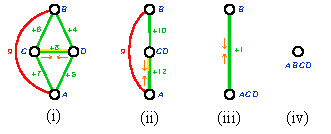
\includegraphics[width=\textwidth]{figs/example_no_constr.pdf}
        \caption{No constraints}\label{subfig:no_constraints}
    \end{subfigure} \hfill
    \begin{subfigure}[t]{0.46 \textwidth}
        \centering
        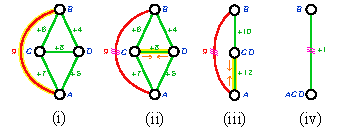
\includegraphics[width=\textwidth]{figs/example_with_constr.pdf}
        \caption{With cannot-link constraints}\label{subfig:with_constraints}
    \end{subfigure}
\caption{Some iterations of the generalized algorithm (using \emph{Sum} linkage criteria) with and without adding cannot-link constraints. The graph has both attractive (green) and repulsive (red) edges and cannot-link constraints are shown with triple violet bars on the edges. We note that when constraints are enforced, the final clustering is given by two clusters instead of only one.}
\label{fig:algorithm_with_without_CLC}
\end{figure}
\begin{algorithm}[t]
  \caption{\algname{}: generalized algorithm for signed graph partitioning}
   \hspace*{\algorithmicindent} \textbf{Input:} Graph $\mathcal{G}(V,E,w^+,w^-)$; linkage criterion $\interact{}$; boolean {\color{blue}\texttt{addCannotLinkConstraints}}  \\
  \hspace*{\algorithmicindent} \textbf{Output:} Final clustering $\Pi$\\
  \hspace*{\algorithmicindent} 
  \begin{algorithmic}[1]
      \State Initialize clustering $\Pi=\{\{v_1\}, \ldots, \{v_{|V|}\}\}$ with each node in its own cluster
      \State Initial interactions between nodes given by $\cost_e = w^+_e - w^-_e$
      \Repeat
        \State Select pair of clusters $S_u,S_v\in\Pi$ with highest absolute interaction $|\interact{}(S_u,S_v)|$
        \If{\big[{\color{ForestGreen}\textbf{$\interact{}(S_u,S_v) > 0$}}\big] \textbf{and} \big[$S_u,S_v$ are \textbf{not} constrained\big]}
          \State Merge cluster $S_u$ with $S_v$: update interactions and cannot-link constraints with all their neighbors
        \ElsIf{\big[{\color{red}\textbf{$\interact{}(S_u,S_v) \leq 0$}}\big] \textbf{and} {\color{blue}\texttt{addCannotLinkConstraints}}}
          \State Add CannotLink Constraint between clusters $S_u$ and $S_v$
        \EndIf
      \Until{\big[all interactions between clusters are repulsive\big] \textbf{or} \big[all adjacent clusters have cannot-link constraints\big]}
      \State
      \Return $\Pi$
  \end{algorithmic}
  \label{main_alg}
\end{algorithm}

\subsection{\algname{}: generalized algorithm for signed graph partitioning} \label{sec:algorithm} 

In Algorithm \ref{main_alg}, we provide simplified pseudo-code for the proposed \algname{} algorithm. \algname{} implements a bottom-up approach that starts by assigning each node to its own cluster and then iteratively merges pairs of adjacent clusters. The algorithm has two variants. The first one, with \texttt{addCannotLinkConstraints=False}, starts by merging clusters with the strongest attractive interaction and stops once the remaining clusters share only mutual repulsive interactions (see iterations on toy graphs in block 4 of Fig. \hyperref[fig:intro_figure]{\ref*{fig:intro_figure}}). After each merging iteration, the interaction between the merged cluster and its neighbors is updated according to one of the linkage criteria $\interact(S_u, S_v)$ listed in Table \ref{tab:linkage-criteria}.

In the second variant, when \texttt{addCannotLinkConstraints=True}, Algorithm \ref{main_alg} also introduces \emph{cannot-link constraints}, which represent mutual exclusion relationships between pairs of nodes that cannot be associated with the same cluster in the final clustering. This variant 
selects the pair of clusters with the highest absolute interaction $|\interact(S_u, S_v)|$, so that the most attractive and the most repulsive pairs are analyzed first (see example in Fig. \ref{subfig:with_constraints}). If the interaction is repulsive, then the two clusters are constrained and its members can never merge in subsequent steps. If the interaction is attractive, then the clusters are merged, provided that they were not previously constrained. 
The algorithm terminates when all the remaining clusters are constrained.

In Appendix \ref{sec:detailed_impl}, we comment on the algorithm's computational complexity $\mathcal{O}(N^2 \log N)$ and present our implementation given by the edge contraction Algorithm \ref{detailed_alg} based on a priority queue.

\begin{table*}[b]
    \centering
    \scriptsize
    \begin{subtable}[t!]{\textwidth}\centering
        \begin{tabular}{c r  l | c | c  c}
            \multicolumn{3}{c|}{\multirow{2}{*}[-0.5em]{\thead{\textbf{\algname{} linkage criteria} $\,\,\interact(S_u ,S_v)$}}}  & \multirow{2}{*}[-0.5em]{\thead{\textbf{Unsigned Graphs}}} & \multicolumn{2}{c}{\thead{\textbf{Signed Graphs}}}  \\        
            \multicolumn{3}{c|}{} &  &  \multicolumn{1}{c}{\thead{No Constraints}} & \thead{With Constraints} \\        
      
            \midrule
             & Sum: & $\displaystyle \sum_{e\in E_{uv}} \cost_e$ & \thead{Sum Linkage\\Hier. Aggl. Clust.} & \thead{GAEC \cite{keuper2015efficient}} & \thead{Greedy Fixation \cite{levinkov2017comparative}} \\ 
            
             &\makecell[r]{Absolute Max:} & 
            $\displaystyle \cost_e$ with $\displaystyle e = \argmax_{t\in E_{uv}} |\cost_t|$
               & \thead{Single Linkage\\Hier. Aggl. Clust.} & \thead{Mutex Watershed \cite{wolf2018mutex}} & \thead{Mutex Watershed \cite{wolf2018mutex}} \\
             & \makecell[r]{Average:} & $\displaystyle \sum_{e\in E_{uv}} \cost_e \bigg/ \big|E_{uv}\big|  $ & \thead{ Average Linkage\\ Hier. Aggl. Clust.} & \thead{\textbf{NEW}} & \thead{\textbf{NEW}}\\ 

            & Max: & $\displaystyle \max_{e\in E_{uv}} \cost_e$ & \thead{Single Linkage\\Hier. Aggl. Clust.} & \thead{\textbf{NEW}} & \thead{\textbf{NEW}}\\ 

            & Min:& $\displaystyle \min_{e\in E_{uv}} \cost_e$ & \thead{Complete Linkage\\ Hier. Aggl. Clust.}  & \thead{\textbf{NEW}} & \thead{\textbf{NEW}}



            
        \end{tabular}
    \end{subtable} 
    \caption{Existing and new clustering algorithms that can be reformulated as special cases of the proposed generalized algorithm for signed graph partitioning \algname{}, given a linkage criterium, a type of graph (signed or unsigned) and the optional use of cannot-link constraints. The set $E_{uv}$ is defined as the set of all edges connecting cluster $S_u$ to cluster $S_v$, i.e. $E_{uv}=(S_u \times S_{v \neq u}) \cap E$.}
    \label{tab:linkage-criteria}
\end{table*}
\begin{figure}
\centering
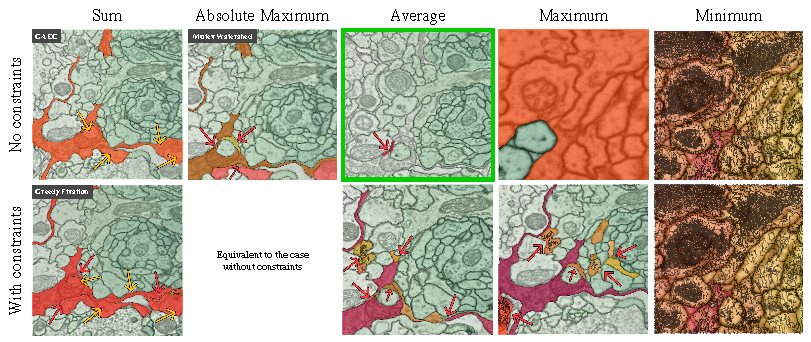
\includegraphics[width=\textwidth]{./figs/comparison_new.pdf} % left bottom right top
\caption{Failure cases of \algname{} with different linkage criteria highlighted on some difficult parts of the CREMI Challenge data. The main \emph{wrongly} segmented regions are highlighted in different warm colors. Note that the data is 3D, hence the same color could be assigned to parts of segments that appear disconnected in 2D.  Red arrows point to wrongly split regions. Yellow arrows point out merge errors. The \emph{Average} linkage without cannot-link constraints returned the best segmentation.
\label{fig:cremi_comparison}}
\end{figure}



\subsection{\algname{} with different linkage criteria: new and existing algorithms} \label{sec:alg_update_rules}

Our main contribution is the generalized algorithm for signed graph partitioning, short GASP, that encompasses several known and novel agglomerative algorithms on display in Table \ref{tab:linkage-criteria}.
In our framework, individual algorithms are differentiated by the linkage criterion employed. We review them in the following paragraphs.

In the special case of an unsigned graph with only positive interactions, i.e. $w_e^-=0$ and $\cost_e \geq 0$ $\forall e\in E$, 
 the algorithm performs a standard agglomerative hierarchical clustering by returning only a single cluster and a hierarchy of clusters defined by the order in which the clusters are merged (see Table \ref{tab:linkage-criteria}, unsigned graphs).

Given a graph with both attractive and repulsive cues, an edge contraction algorithm with a sum update rule was pioneered in \cite{levinkov2017comparative,keuper2015efficient} (Table \ref{tab:linkage-criteria}, \emph{Sum} linkage). The authors present both a version with cannot-link constraints and one without, and then compare them with other greedy local-search algorithms approximating the multicut optimization problem.
The Mutex Watershed \cite{wolf2018mutex} is another signed graph partitioning algorithm that introduces dynamical cannot-link constraints. In Proposition \ref{prop:equiv_MWS} (see Appendix \ref{sec:appendix_abs_max}) we prove that, surprisingly, it can also be seen as an efficient implementation of \algname{} with \emph{Absolute maximum} linkage (def. in Table \ref{tab:linkage-criteria}). Moreover, in Proposition \ref{prop:abs_max_cannot_link_property} we also prove that \algname{} with \emph{Abs Max} linkage returns the same clustering with or without enforcing cannot-link constraints.
On the other hand, to our knowledge, \emph{Average}, \emph{Max} or \emph{Min} linkage criteria have never been used for signed graph agglomerative algorithms or been combined with cannot-link constraints.

Apart from the linkage criteria defined in Table \ref{tab:linkage-criteria}, additional ones were proposed in the literature:
\cite{nunez2013machine} for example uses a learned approach where a random forest classifier updates the cluster interactions depending on predefined edge and node features; other approaches introduce a weight regularization depending on the size of the clusters \cite{felzenszwalb2004efficient,kardoostsolving}, whereas 
\cite{funke2018large} uses a \emph{quantile} linkage criteria by populating a histogram for each inter-cluster interaction. In our experiments, we decided to focus on the linkage criteria listed in Table \ref{tab:linkage-criteria}, since they represent the most common options.

